\documentclass[11pt]{article}

% ====== Packages ======
\usepackage[T1]{fontenc}
\usepackage[utf8]{inputenc}  % if you use XeLaTeX/LuaLaTeX, remove this and set fonts directly
\usepackage{lmodern}
\usepackage{microtype}
\usepackage[margin=1in]{geometry}
\usepackage{setspace}
\usepackage{xcolor}
\usepackage{graphicx}
\usepackage{subcaption}
\usepackage{booktabs}
\usepackage{siunitx}
\usepackage{amsmath,amssymb}
\usepackage{enumitem}
\usepackage{hyperref}
\usepackage[capitalize,noabbrev]{cleveref}
\usepackage{listings}
\usepackage{caption}

% ====== Listings (code) style ======
\lstdefinestyle{mystyle}{
  basicstyle=\ttfamily\small,
  frame=single,
  breaklines=true,
  columns=fullflexible,
  numbers=left,
  numberstyle=\tiny,
  xleftmargin=1.5em,
  showstringspaces=false
}
\lstset{style=mystyle}

% ====== Hyperref colors ======
\hypersetup{
  colorlinks=true,
  linkcolor=blue!50!black,
  citecolor=blue!50!black,
  urlcolor=blue!50!black
}

% ====== Clever helpers ======
\newcommand{\etal}{\textit{et~al.}}
\newcommand{\ie}{i.e., }
\newcommand{\eg}{e.g., }

% ====== Project knobs (edit here to reflect final runs) ======
\newcommand{\NumRoutersA}{64}         % 4x4x4
\newcommand{\NumRoutersB}{64}         % 8x8 (2D baseline with same count)
\newcommand{\Ruby}{Garnet 3.0}
\newcommand{\SimCycles}{2{,}000{,}0}
\newcommand{\Clk}{2\,GHz}
\newcommand{\LinkW}{128\,bits}
\newcommand{\LinkLat}{1}              % ticks
\newcommand{\RouterLat}{1}            % ticks

\title{\textbf{Toward Practical 3D NoCs: Topology Design, Routing Bias, and Cost--Performance Trade-offs}\\
\large A gem5/\Ruby\ Study of 3D Mesh and Sparse-Vertical Variants}
\author{Your Name \quad Your Collaborator\\[2pt]
\small Institution / Course / Term}
\date{\today}

\begin{document}
\maketitle
\doublespacing

\begin{abstract}
While 2D Network-on-Chip (NoC) fabrics are mature and widely deployed, industry is actively exploring 3D NoC organizations to unlock higher bisection bandwidth and lower hop counts without growing chip footprint. Using \texttt{gem5} with \Ruby, we first reproduce the well-known efficiency advantage of a 3D Mesh against a 2D Mesh with the \emph{same number of routers} (e.g., \NumRoutersA\ vs.\ \NumRoutersB). However, dense per-router TSV columns exacerbate manufacturing yield risks and area/power overhead, as reported by prior cluster mesh studies. Motivated by these practical constraints, we implement several 3D topologies with \emph{sparser Z connectivity}: (i) Cluster3D with hub-based vertical sharing, (ii) Sparse3D Pillars, (iii) 3D Small-World Express links, and (iv) Hierarchical 3D Chiplets. We provide configurable Python topologies, weight-based TABLE routing to bias paths, and a measurement methodology. Our experiments sweep injection rates across traffic patterns, exposing how each design trades off performance (latency/throughput) versus TSV budget and routing simplicity. 
\end{abstract}

\section{Introduction}
2D NoCs have benefited from years of architectural optimization and tooling. As transistor scaling slows and multi-die integration rises, 3D NoCs promise better path lengths and bandwidth density. Yet, deploying dense vertical connections (TSVs or micro-bumps) at each router often faces yield, cost, and thermal constraints. As a result, practical systems seek \emph{structured sparsity} in the Z dimension: not every router needs its own vertical link, so long as the network can route efficiently to shared vertical resources.

This project asks: \emph{(1) How much efficiency do we retain when we replace a fully dense 3D Mesh with more practical, sparse-Z topologies? (2) Which sparse patterns strike the best balance between performance and implementation cost?} We build four representative families in \texttt{gem5}/\Ruby\ and evaluate them against classic 3D/2D Mesh baselines.

\paragraph{Contributions.}
\begin{itemize}[leftmargin=1.2em]
  \item A clean set of \texttt{configs/topologies} for 3D Mesh and three sparse-Z designs (Cluster3D-Hub, Sparse3D-Pillars, SW3D-Express) plus a hierarchical 3D Chiplet fabric.
  \item Weight-based TABLE routing schemes that bias traffic toward designated vertical conduits or express links while preserving deadlock freedom.
  \item A reproducible measurement pipeline (sweeps, CSV collection, plotting) to compare latency, throughput, link utilization, and saturation points under uniform and non-uniform traffic.
  \item Case studies of cost--performance trade-offs under fixed ``vertical budget,'' highlighting where sparse designs approach dense mesh performance.
\end{itemize}

\section{Background and Related Work}
\subsection{Dense 3D Mesh vs.\ 2D Mesh}
3D Mesh reduces average hop count by adding Z edges to the 2D grid, which can improve latency and throughput at a fixed router count. We briefly review dimension-order routing (DOR) and weight-based TABLE routing in \Ruby, and how link/router latencies model physical effects.

\subsection{Manufacturability and TSV Economics}
Prior work (e.g., cluster mesh proposals) notes that a TSV per router can hurt yield and area. We discuss TSV pitch, thermal implications, and common mitigations (sharing, pillars, chiplets).

\subsection{Sparse-Vertical and Hierarchical 3D Fabrics}
We summarize key ideas behind: hub-sharing (Cluster3D), pillar-based sparsity, small-world express links, and chiplet-level hierarchies, motivating our four concrete designs.

\section{Topologies Implemented}
This work adds Python topologies under \texttt{configs/topologies/}. All use \texttt{IntLink}/\texttt{ExtLink} wiring with explicit port names (e.g., \texttt{East}, \texttt{UpGW}, \texttt{EastExp}) and \emph{weights} to guide TABLE routing.

\subsection{3D Mesh (XYZ DOR baseline)}
\label{sec:mesh3d}
We use a standard 3D Mesh (e.g., $4{\times}4{\times}4$) with fully populated Z links and DOR (XYZ) or TABLE routing with $W_X < W_Y < W_Z$.
\begin{itemize}[leftmargin=1em]
  \item \textbf{Goal}: establish the upper-bound efficiency for a given router count.
  \item \textbf{parameters}: link/router latency=1; vc = 4 (default); sim-cycle = 20000; link-width=128; GlobalFrequency=2GHz.
\end{itemize}
\begin{figure}[htbp]
    \centering
    \begin{subfigure}[t]{0.45\linewidth}
        \centering
        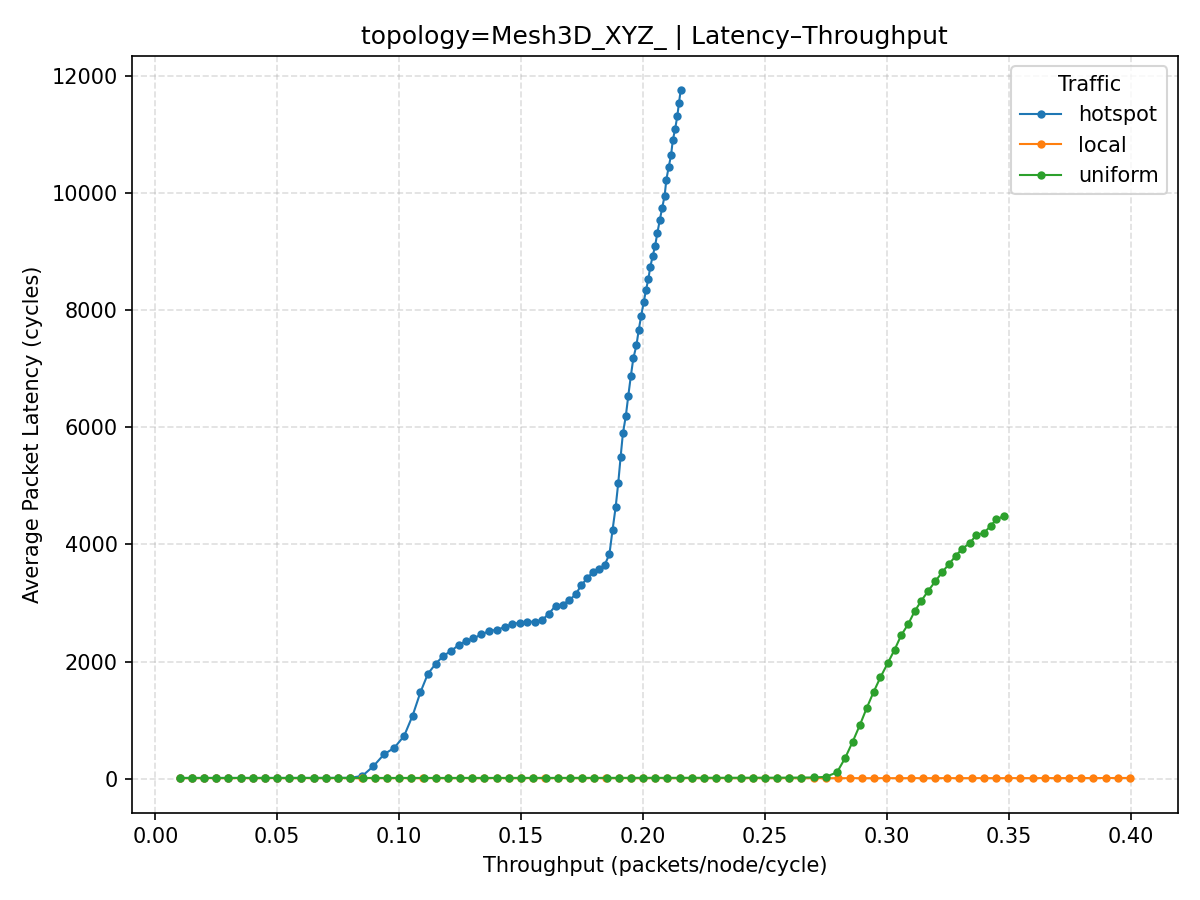
\includegraphics[width=\linewidth]{./figs/Mesh3D-traffic.png}
        \caption{Throughput of the 3D Mesh topology under varying injection rates across different traffic patterns. Uniform traffic achieves the highest sustained throughput, while hotspot traffic saturates earlier due to localized congestion. Local traffic benefits from short paths and maintains high efficiency.}
        \label{fig:mesh3d-throughput}
    \end{subfigure}
    \hfill
    \begin{subfigure}[t]{0.45\linewidth}
        \centering
        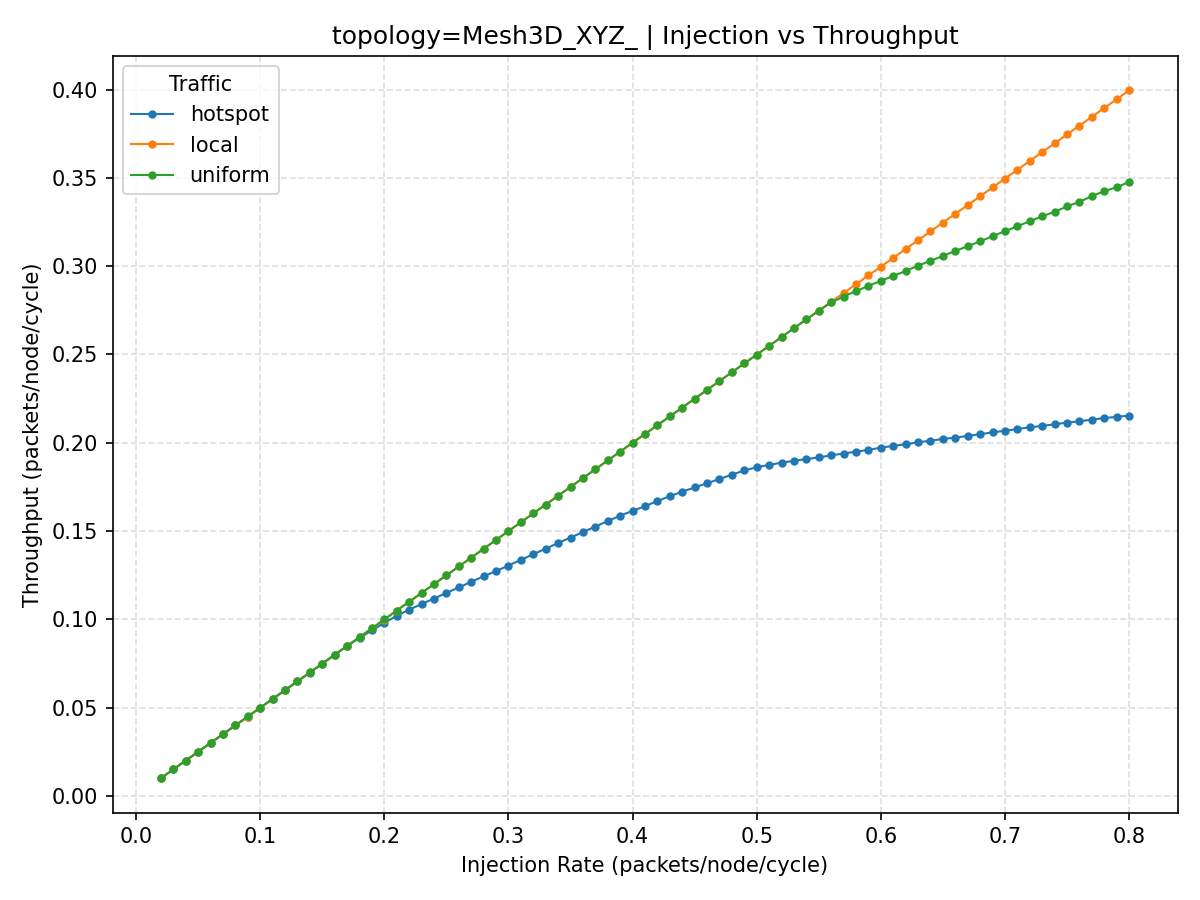
\includegraphics[width=\linewidth]{./figs/Mesh3D-inj_rate-throughput.png}
        \caption{Average packet latency versus throughput for the 3D Mesh network. At low loads, latency remains low; however, as the network approaches saturation, hotspot traffic experiences a sharp rise in latency, while uniform traffic maintains stability up to higher throughput levels.}
        \label{fig:mesh3d-latency-throughput}
    \end{subfigure}
    \caption{Performance evaluation of the 3D Mesh topology under three canonical traffic patterns: (a) throughput vs.\ injection rate, and (b) latency-throughput trade-off. Results demonstrate that although 3D Mesh offers strong baseline performance, its behavior varies significantly with traffic distribution, especially under congestion.}
    \label{fig:mesh3d-performance}
\end{figure}

\subsection{Cluster3D\_Hub}
A $2{\times}2$ submesh per layer shares a central hub; hubs connect vertically. The hub is transit-only (no endpoint injection). We bias routes via weights to funnel local traffic through its hub for Z.
\begin{itemize}[leftmargin=1em]
  \item \textbf{Design knobs}: cluster size (e.g., $2{\times}2{\times}1$, $2{\times}2{\times}2$), vertical speedup, hub router latency reduction.
  \item \textbf{Rationale}: cut TSV count while preserving short detours to vertical resources.
\end{itemize}

\subsection{Sparse3D\_Pillars}
Place vertical pillars every $(P_x, P_y)$ tiles. Only routers aligned to a pillar get Up/Down links. Traffic uses XY detours to the nearest pillar, then moves vertically.
\begin{itemize}[leftmargin=1em]
  \item \textbf{Design knobs}: $P_x,P_y$ spacing, aligned vs.\ staggered patterns (future work).
  \item \textbf{Routing}: TABLE with $W_X<W_Y<W_Z$ and no direct Up/Down from non-pillar routers.
\end{itemize}

\subsection{SW3D\_Express}
Add a budget of long-range \emph{express} links (in-plane or cross-layer) on top of 3D Mesh or sparse-Z base. We use special port names (\texttt{EastExp}, \texttt{UpExp}, \ldots) and assign them the lowest weight ($W_{\text{EXP}}$).
\begin{itemize}[leftmargin=1em]
  \item \textbf{Design knobs}: grid-based placement period $K$ (rule-based); total budget $B$; (optional) randomized placement.
  \item \textbf{Routing}: TABLE prefers express edges first, then normal links.
\end{itemize}

\subsection{Hier3D\_Chiplet}
Partition the die into chiplets (e.g., $4{\times}4{\times}1$ each). Within a chiplet: local mesh. Gateways (1--2 per chiplet) connect to a backbone (2D in-layer and/or vertical). Gateways use \texttt{*GW} ports and higher weights at the backbone to avoid overuse.
\begin{itemize}[leftmargin=1em]
  \item \textbf{Design knobs}: chiplet dimensions, \#gateways, backbone topology (ring/mesh), vertical gateway connectivity.
  \item \textbf{Routing}: TABLE with tiered weights: $W_{\text{intra}} < W_{\text{backbone}} < W_Z$.
\end{itemize}

\begin{table}[t]
  \centering
  \caption{Topology summary and intended routing bias (lower weight is preferred). Edit with your final parameters.}
  \label{tab:topo-summary}
  \begin{tabular}{lcccc}
    \toprule
    \textbf{Topology} & \textbf{Z budget} & \textbf{Extra links} & \textbf{Routing mode} & \textbf{Weights (X/Y/Z/extra)} \\
    \midrule
    3D Mesh         & dense & none      & TABLE or XYZ DOR & 1/2/3/-- \\
    Cluster3D\_Hub  & sparse hubs & hub vertical & TABLE & 1/2/3/-- (hub Z sped-up) \\
    Sparse3D\_Pillars & pillars $(P_x,P_y)$ & none & TABLE & 1/2/3/-- \\
    SW3D\_Express   & dense/sparse & express & TABLE & 1/2/3/0 (exp) \\
    Hier3D\_Chiplet & per-gateway & backbone & TABLE & 1/2/3/-- (+GW tier) \\
    \bottomrule
  \end{tabular}
\end{table}

\section{Routing and Deadlock Considerations}
We primarily use TABLE-based routing in \Ruby\ with weights to induce preferences:
\begin{itemize}[leftmargin=1em]
  \item \textbf{Strict ordering}: Distinct weights per dimension/tier maintain a partial order and avoid cycles typical in oblivious shortest-path selection.
  \item \textbf{Express edges}: assign the smallest weight (e.g., $W{=}0$) to let the router choose them deterministically before normal links.
  \item \textbf{Gateway tiers}: use intermediate weights for backbone/GW hops to avoid accidental oscillations.
\end{itemize}
We validated reachability via \texttt{config.ini} inspections and by eliminating ``No Route exists from this Router'' fatals during warmup runs.

\section{Methodology}
\subsection{Simulator and Network}
We use \texttt{gem5}  with \Ruby\ (Garnet 3.0). Unless noted, system and Ruby clocks are 2GHz. Link width \LinkW, link latency \LinkLat, router latency \RouterLat.



\subsection{Metrics}
We collect average packet/flit latency, average hops, total injected/received packets (to derive accepted rate), and average link utilization. Saturation is indicated by the knee where latency diverges and accepted rate flattens.

\section{Experimental Results}
In following experiments, we use transpose traffic patterns to simulate hotspot traffic, and use neighbor traffic patterns to simulate local traffic, and uniform-random is identical to uniform traffic.
\subsection{3D Mesh vs.\ 2D Mesh (same router count)}
\label{sec:mesh-baseline}

We compare a $4{\times}4{\times}4$ 3D Mesh with an $8{\times}8$ 2D Mesh, both using \NumRoutersA\ routers and identical link/router latencies. The 3D topology is expected to achieve lower average hop counts and higher throughput due to shorter paths and improved bisection bandwidth.

As shown in \cref{fig:mesh-comparison-full}, the 3D Mesh supports significantly higher throughput before saturation under uniform and transpose traffic (up to $\sim$0.35 packets/node/cycle), compared to the 2D Mesh's saturation at $\sim$0.21. Moreover, the 3D design reduces average hop count—especially under uniform traffic—from $\sim$5.3 in 2D to $\sim$3.75 in 3D—by leveraging vertical shortcuts.
\begin{figure}[htbp]
    \centering
    \begin{subfigure}[t]{0.45\linewidth}
        \centering
        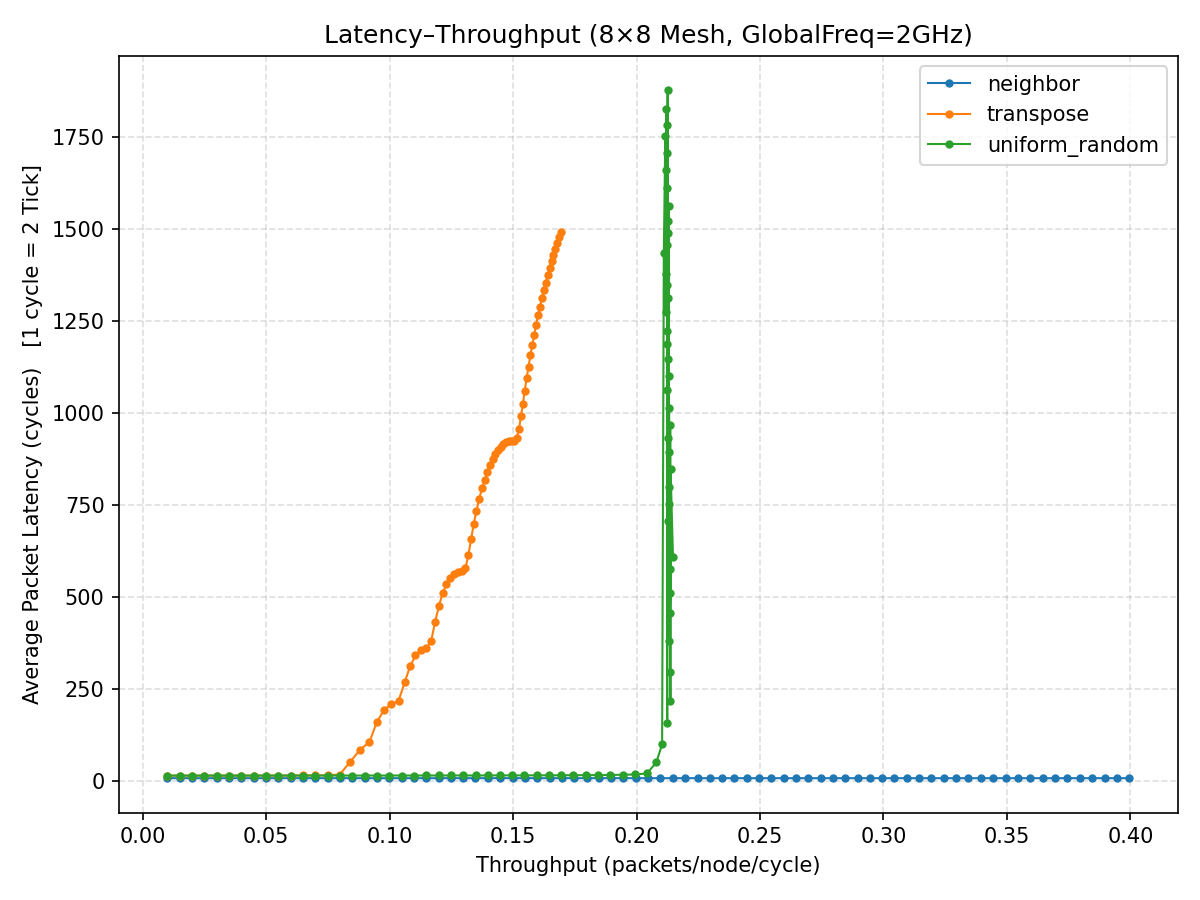
\includegraphics[width=\linewidth]{./figs/Mesh2D-traffic.png}
        \caption{Latency-throughput curve for the $8{\times}8$ 2D Mesh under uniform, transpose, and neighbor traffic patterns. The network saturates at approximately 0.21 packets/node/cycle, with latency diverging sharply under uniform and transpose traffic due to global congestion. Neighbor traffic remains stable due to short paths.}
        \label{fig:mesh2d-latency-throughput}
    \end{subfigure}
    \hfill
    \begin{subfigure}[t]{0.45\linewidth}
        \centering
        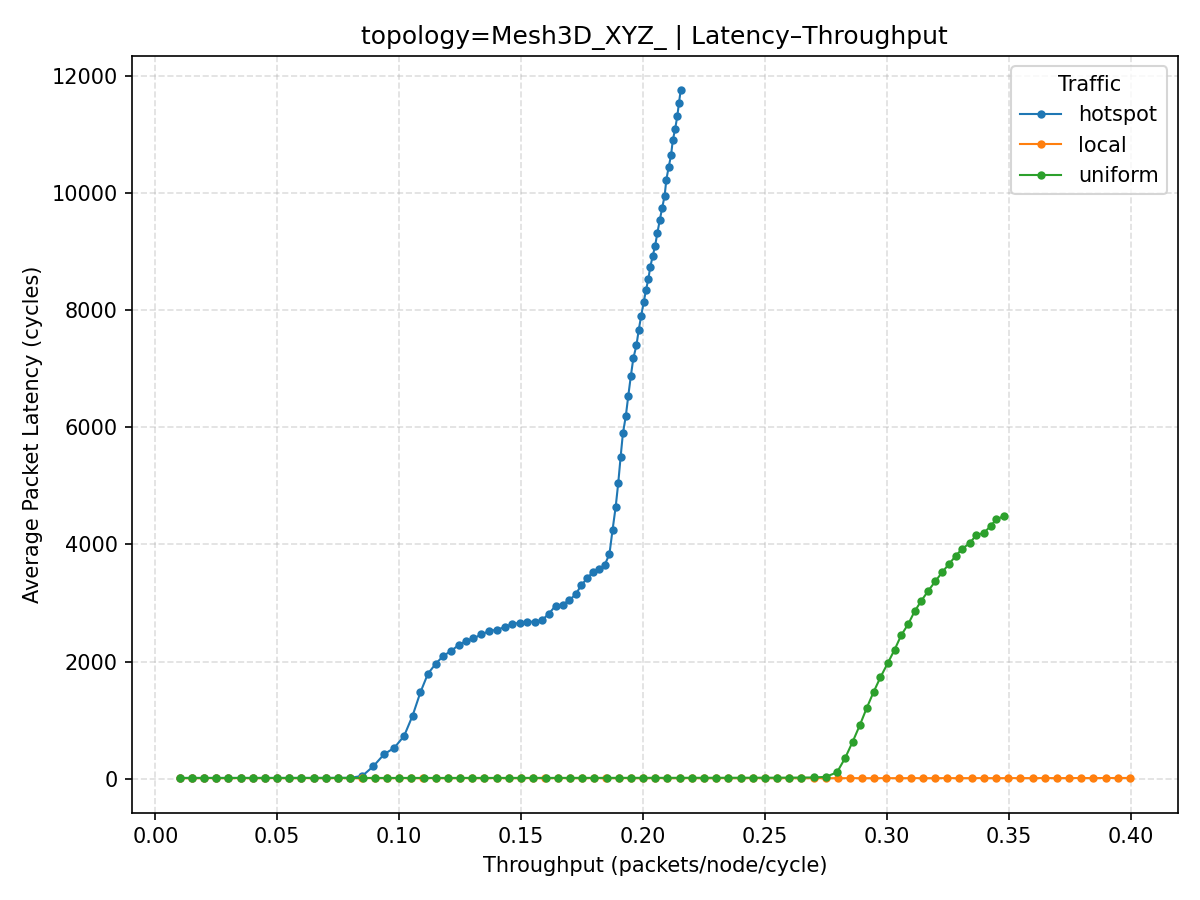
\includegraphics[width=\linewidth]{./figs/Mesh3D-traffic.png}
        \caption{Latency-throughput curve for the $4{\times}4{\times}4$ 3D Mesh under hotspot, local, and uniform traffic. Despite higher average hop counts in some cases, the 3D topology achieves significantly higher throughput before saturation (up to $\sim$0.35), especially under uniform traffic, thanks to reduced path lengths and better bisection bandwidth.}
        \label{fig:mesh3d-latency-throughput}
    \end{subfigure}
    
    \vspace{1em} % 添加垂直间距
    
    \begin{subfigure}[t]{0.45\linewidth}
        \centering
        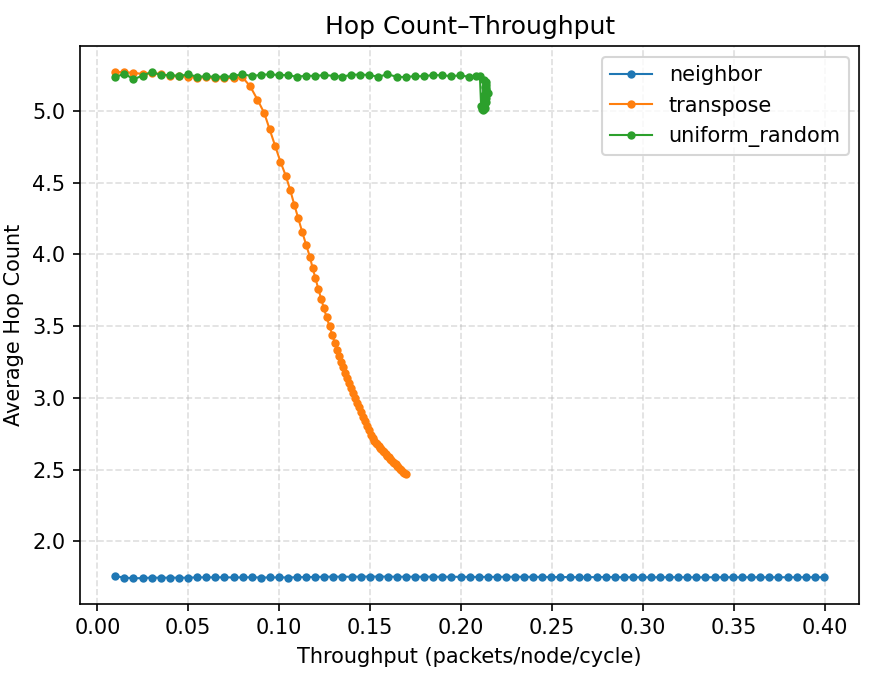
\includegraphics[width=\linewidth]{./figs/Mesh2D_throughput_hops.png}
        \caption{Average hop count versus throughput for the $8{\times}8$ 2D Mesh. Neighbor traffic maintains a constant low hop count ($\sim$1.7) due to short distances. Transpose traffic shows a sharp drop in hop count as injection rate increases, indicating more efficient routing through balanced load distribution. Uniform traffic remains near the theoretical maximum of 5.3 hops across all loads, reflecting long, random paths.}
        \label{fig:mesh2d-hops}
    \end{subfigure}
    \hfill
    \begin{subfigure}[t]{0.45\linewidth}
        \centering
        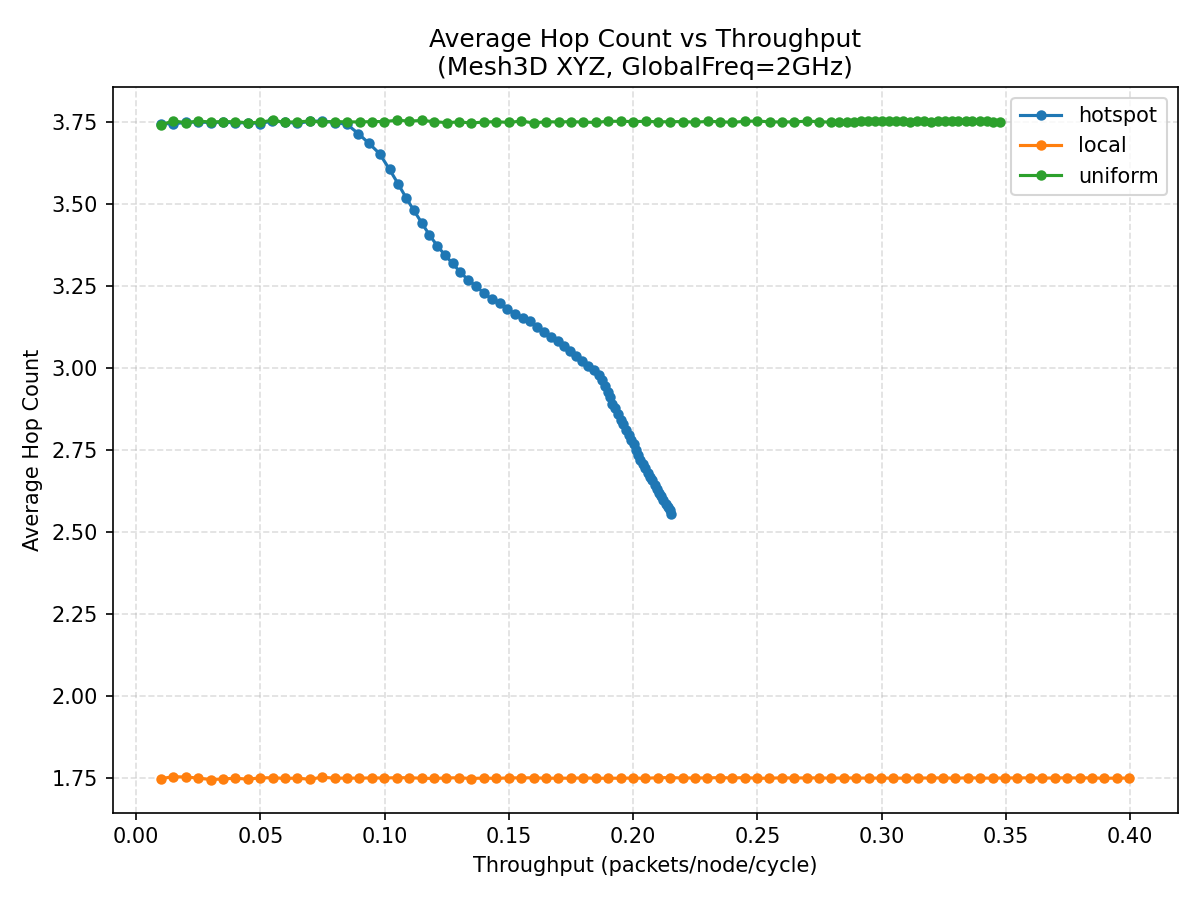
\includegraphics[width=\linewidth]{./figs/Mesh3D_throughput_hops.png}
        \caption{Average hop count versus throughput for the $4{\times}4{\times}4$ 3D Mesh. Local traffic maintains a minimal hop count ($\sim$1.75) throughout, consistent with its short-range nature. Hotspot traffic exhibits a gradual decrease in hop count with increasing load, suggesting adaptive routing or load-balancing effects. Uniform traffic stabilizes at $\sim$3.75 hops, which is significantly lower than the 2D baseline, demonstrating the benefit of Z-dimension shortcuts in reducing average path length.}
        \label{fig:mesh3d-hops}
    \end{subfigure}
    
    \caption{Comparison of performance metrics between 2D Mesh ($8{\times}8$) and 3D Mesh ($4{\times}4{\times}4$) with identical router count (\NumRoutersA). Top row: latency-throughput curves show that the 3D Mesh supports higher throughput and earlier saturation under global workloads. Bottom row: hop count trends reveal that the 3D Mesh reduces average path length, especially under uniform traffic, by leveraging vertical links for shorter routes.}
    \label{fig:mesh-comparison-full}
\end{figure}

\subsection{Effect of Escape VC on 3D vs. 2D}
\label{subsec:escape-vc}
We repeat the uniform-random sweep while enabling an \emph{escape virtual channel} (VC$_0$) reserved for a strictly ordered, deadlock-free route set (e.g., DOR). The remaining VCs use the standard (normal/adaptive) policy. \textbf{All other parameters are kept identical} across 2D and 3D (\texttt{vcs-per-vnet}=4 with one reserved for escape, identical buffers, link/router latencies, clocks, and traffic).


Empirically, the 2D Mesh exhibits a clear knee (threshold throughput) around $\sim$0.21 pkts/node/cycle, whereas the 3D Mesh shows no visible knee up to our maximum offered load of 0.7, achieving accepted throughput $\geq$0.35 in the sweep. Using the \emph{threshold throughput} metric, the relative advantage of 3D increases from about 35\% (without escape VC) to \textbf{$\geq$50--60\%} with escape VC (e.g., $0.35/0.21\approx1.67\times$).


\begin{figure}[htbp]
  \centering
  \begin{subfigure}[t]{0.48\linewidth}
    \centering
    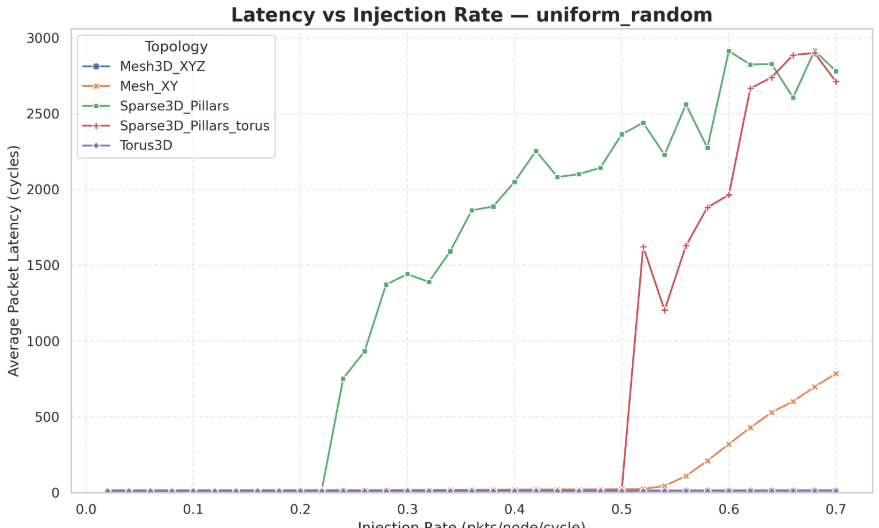
\includegraphics[width=\linewidth]{./figs/escape_lat_vs_inj.png}% TODO: replace with your actual filename
    \caption{Latency vs. injection under uniform-random with escape VC.}
  \end{subfigure}\hfill
  \begin{subfigure}[t]{0.48\linewidth}
    \centering
    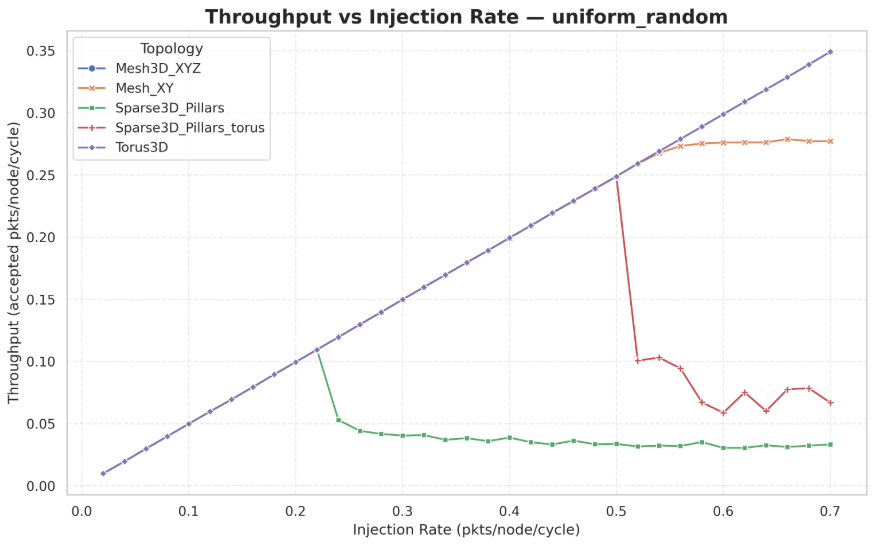
\includegraphics[width=\linewidth]{./figs/escape_thr_vs_inj.png}% TODO: replace with your actual filename
    \caption{Accepted throughput vs. injection under uniform-random with escape VC.}
  \end{subfigure}
  \caption{Escape VC (VC$_0$) amplifies the 3D advantage: 2D shows a knee near $\sim$0.21, while 3D shows no knee up to $\geq$0.35 within our sweep range.}
  \label{fig:escape-vc-results}
\end{figure}


\paragraph{Intuition.} The escape VC guarantees progress, allowing the other VCs to exploit additional turn freedom and transient path diversity. In 3D, the Z dimension supplies more minimal and near-minimal alternatives, so adaptive VCs more effectively relieve head-of-line blocking and allocator contention than in 2D.


\paragraph{Fairness and limits.} Both 2D and 3D reserve exactly one escape VC; buffer sizes and VC counts per input port are identical. Our current sweep upper bound is 0.7 offered load; future work will extend the range to locate the 3D knee more precisely.

\subsection{Sparse-Z Designs under a Fixed Vertical Budget}
\label{sec:sparse-results}
We normalize each design to a comparable TSV count (or pillar density) and evaluate:
\begin{itemize}[leftmargin=1em]
  \item Latency/throughput curves across traffic patterns.
  \item Avg.\ link utilization and hop distributions.
  \item Sensitivity to vertical speedup and gateway count.
\end{itemize}


\subsection{Ablations}
\paragraph{Cluster size \& hub speedup.} How 2x2 vs.\ 3x3 clusters and hub DVFS change the knee point.
\paragraph{Pillar spacing $(P_x,P_y)$.} Trade-offs between detour cost and TSV count.
\paragraph{Express budget $B$ and period $K$.} Diminishing returns of additional long links.
\paragraph{Chiplet gateways.} One vs.\ two gateways per chiplet and backbone shape.

\section{Discussion}
\subsection{Which Sparse Pattern Scales Best?}
We interpret the results through the lens of manufacturing and thermal feasibility, highlighting topologies that get “close enough” to dense 3D Mesh while using far fewer vertical links.

\subsection{Routing Simplicity vs.\ Performance}
TABLE routing with weights gives strong baselines without custom algorithms; we note when custom adaptive schemes might help (left as future work).

\subsection{Limitations}
Cycle-accurate microarchitectural models (buffers, VC allocation) follow Garnet defaults; real silicon may differ in timing closure and power. Our synthetic traffic stresses the network but does not model specific workloads.

\section{Conclusion}
3D NoCs are promising, but dense Z wiring is difficult to manufacture at scale. Our study shows that structured sparsity—hub sharing, pillars, express links, and chiplets—retains much of the performance benefit while substantially reducing vertical resources. Weight-based TABLE routing is a practical mechanism to guide traffic along these sparse conduits.

\appendix

\section{Topology Implementation Details}
We place our Python files in \texttt{configs/topologies/}: 
\begin{itemize}[leftmargin=1em]
  \item \texttt{Mesh3D\_XYZ\_.py}: 3D Mesh baseline (XYZ DOR or TABLE).
  \item \texttt{Cluster3D\_Hub.py}: cluster hub + vertical hub links (with configurable hub speedup).
  \item \texttt{Sparse3D\_Pillars.py}: pillar spacing $(P_x,P_y)$; optional staggered layout (future).
  \item \texttt{SW3D\_Express.py}: rule-based express placement (period $K$) with $W_{\text{EXP}}{=}0$.
  \item \texttt{Hier3D\_Chiplet.py}: chiplet size, \#gateways, backbone wiring.
\end{itemize}
We followed gem5’s \texttt{Mesh\_XY} style: create routers, wire \texttt{ExtLink}s to NIs, then build \texttt{IntLink}s with port names and weights.

\section{Command Lines and Sweeps}
\subsection*{Single Run Example}
\begin{lstlisting}[language=bash]
./build/NULL/gem5.opt configs/example/garnet_synth_traffic.py \
  --network=garnet --topology=Sparse3D_Pillars \
  --num-cpus=64 --num-dirs=64 --mesh-rows=4 \
  --routing-algorithm=0 \
  --synthetic=uniform_random --injectionrate=0.05 \
  --sim-cycles=2000000 \
  --sys-clock=1GHz --ruby-clock=1GHz \
  --link-width-bits=128 --link-latency=2 --router-latency=2 \
  --mem-type=SimpleMemory --mem-channels=64 --mem-size=8192MB
\end{lstlisting}

\subsection*{Sweep Script (bash)}
\begin{lstlisting}[language=bash]
for r in $(seq 0.01 0.01 0.25); do
  ./build/NULL/gem5.opt \
    -d runs/pillars_uniform_r${r} \
    configs/example/garnet_synth_traffic.py \
    --network=garnet --topology=Sparse3D_Pillars \
    --num-cpus=64 --num-dirs=64 --mesh-rows=4 \
    --routing-algorithm=0 \
    --synthetic=uniform_random --injectionrate=${r} \
    --sim-cycles=2000000 \
    --sys-clock=1GHz --ruby-clock=1GHz \
    --link-width-bits=128 --link-latency=2 --router-latency=2 \
    --mem-type=SimpleMemory --mem-channels=64 --mem-size=8192MB
done
\end{lstlisting}

\section{Data Collection and Plotting}
\label{sec:repro}
\paragraph{Collect CSV.}
\begin{lstlisting}[language=bash]
./collect.sh runs results/pillars_uniform.csv
\end{lstlisting}

\paragraph{Plot curves.}
\begin{lstlisting}[language=bash]
python3 plot_metrics.py \
  --out results/plots \
  --series "Pillars:results/pillars_uniform.csv" \
  --series "3D Mesh:results/mesh3d_uniform.csv"
\end{lstlisting}

\section{Sanity Checks}
We grep \texttt{config.ini} to confirm topology name, routing mode, \#IntLinks, port names (e.g., \texttt{UpGW}, \texttt{EastExp}) and weight histograms; we ensure every router has outgoing \texttt{IntLink}s.

\section*{References}
\bibliographystyle{abbrv}
\bibliography{references}
\end{document}
